Bayesian statistics offers a powerful framework for modeling uncertainty and performing probabilistic inference, making it particularly well-suited for rare-event searches such as $0 \nu \beta \beta$ decay. 
In this chapter, we explain the essential principles of Bayesian inference and present the statistical model used to estimate the experimental sensitivity for $0 \nu \beta \beta$ decay discovery under a background-only hypothesis and varying pulse shape discrimination efficiencies. 
We do not apply the likelihood model (equation~\refeq{eq:bayes_likelihood}) directly to real data. Although the LEGEND-200 data in the $(Q_{\beta \beta} \pm 25)$~keV window has been unblinded, waveform-level information is not accessible to the full collaboration. Instead, we estimate the expected 90\% credible upper limit on the signal half-rate, defined as the inverse of the signal half-life (see equation~\refeq{eq:signal_half_rate}), using toy Monte Carlo datasets. The usage of half-rate $\mathcal{S} = 1 / T^{0 \nu}_{1/2}$ instead of half-life improves numerical stability. 
To this end, we generate toy spectra and fit them using a signal-plus-background model within a Markov Chain Monte Carlo framework. From the resulting posterior distributions, we derive upper limits on the signal half-rate and define the experimental sensitivity as the median of the 90\% credible interval (CI) distributions. We also detail the fit procedure, including the treatment of nuisance parameters. 


\subsection{Introduction to Bayesian inference}

Bayes' theorem forms the foundation of Bayesian inference, providing a formal mechanism for updating probabilistic beliefs based on observed data:

\begin{equation}
\label{eq:bayes_theorem}
	p(\boldsymbol{\theta} \mid \mathrm{data}) = \frac{p(\mathrm{data} \mid \boldsymbol{\theta}) \cdot p(\boldsymbol{\theta})}{p(\mathrm{data})} \,.
\end{equation}

\noindent Here, $p(\boldsymbol{\theta})$ denotes the prior distribution, which encodes our prior knowledge or assumptions about the parameters before observing any data. The likelihood $p(\mathrm{data} \mid \boldsymbol{\theta})$ quantifies how probable the observed data is under a given choice of parameters. The resulting posterior distribution $p(\boldsymbol{\theta} \mid \mathrm{data})$ reflects the updated knowledge after accounting for the observed data. If the parameters $\boldsymbol{\theta} = (\theta_1, \theta_2, \ldots, \theta_n)$ are independent, the posterior becomes:

\begin{equation}
\label{eq:bayes_theorem_indep}
	p(\boldsymbol{\theta} \mid \mathrm{data}) = \frac{p(\mathrm{data} \mid \boldsymbol{\theta}) \cdot \prod_{i=1}^n p(\theta_i)} {p(\mathrm{data})} \,.
\end{equation}

This factorization is an approximation that holds only if the parameters are uncorrelated under the prior. In practice, some parameters may exhibit correlations, and modeling their joint prior distribution may be necessary to accurately capture posterior dependencies.
The normalization factor, $p(\mathrm{data})$, known as marginal likelihood, ensures the posterior is normalized:

\begin{equation}
\label{eq:bayes_theorem_normalization}
	p(\mathrm{data}) = \int_{\theta} p(\theta) p(\mathrm{data} \mid \theta) \, d\theta \,.
\end{equation}

This integral marginalizes over all possible values of $\theta$, weighted by their prior probabilities. Marginalization is particularly useful to extract the distribution for a given parameter by integrating out the joint distribution over the unknowns that are not of interest. We later apply it to remove nuisance parameters -- quantities that affect the model but are not of direct interest~\cite{gelman_bayesian_2014}. 

Once the posterior distribution is obtained, it can be used to make predictions about new or unseen data via the posterior predictive distribution. It describes the distribution of potential future observations from a repeated experiment conducted under identical conditions:

\begin{equation}
	p(y \mid \mathrm{data}) = \int p(y, \theta \mid \mathrm{data}) \, d\theta = \int p(y \mid \theta) p(\theta \mid \mathrm{data}) \, d\theta \,.
\end{equation}

\noindent Here, $y$ represents a hypothetical data, $\theta$ are the model parameters, and $p(y \mid \theta)$ is the likelihood of observing $y$ given those parameters. The posterior distribution $p(\theta \mid \mathrm{data})$ captures what we have learned about $\theta$ from the observed data.  

Posterior predictive studies are particularly useful for model checking and sensitivity analysis, as they naturally incorporate uncertainty in the model parameters. They are often used to compare the posterior predictive distribution to newly observed data, because this provides insight into how the model and prior assumptions align with reality. If the original data were modeled appropriately, then the generated values of $y$ under the model should exhibit a distribution similar to that of the observed data.


\subsection{Statistical model for sensitivity estimation}
\label{sec:05_stat_model}


To evaluate the effect of the different PSD efficiencies on the half-life sensitivity of the $0 \nu \beta \beta$ decay, we perform a Bayesian sensitivity study using toy Monte Carlo datasets generated under the null hypothesis (background-only scenario). The $0 \nu \beta \beta$ decay analysis is performed over the energy range from 1930 to 2190~keV. 
Two $\gamma$-lines at $(2104 \pm 5)$~keV and $(2119 \pm 5)$~keV are excluded, resulting in a net analysis window of 240~keV~\cite{gerda_collaboration_final_2020}. The expected number of $0 \nu \beta \beta$ decay events in toy MC datasets, as a function of the signal half-rate $\mathcal{S} = 1/T^{0 \nu}_{1/2}$, is given by:


\begin{equation}
\label{eq:0vbb_signal_counts}
	s \left( \mathcal{S} \right) =  \frac{\log{2} \cdot \mathcal{E} \cdot N_A \cdot \epsilon}{m_{\mathrm{mol}}} \cdot \mathcal{S} = \frac{\log{2} \cdot \mathcal{E} \cdot N_A \cdot \epsilon}{m_{\mathrm{mol}}} \cdot \frac{1}{T_{1/2}} \,.
\end{equation}

Here, we have the following parameters~\cite{agostini_background-free_2017}:

\begin{itemize}
    \item $\mathcal{E} = 1000 \;\mathrm{kg} \cdot {\mathrm{yr}}$ is the exposure
    \item $N_A = 6.022 \times 10^{23} \; \mathrm{mol}^{-1}$ is Avogadro's number
    \item $\epsilon$ is the detection efficiency, calculated as in equation~\refeq{eq:total_efficiency}
    \item $m_{\mathrm{mol}} = 75.92$ g/mol is the molar mass of $^{76}$Ge 
    \item $T^{0 \nu}_{1/2}$ is the $0 \nu \beta \beta$ decay half-life
\end{itemize}

\noindent The number of background events $b$ is given by:


\begin{equation}
\label{eq:0vbb_background_counts}
	b \left( \mathcal{B} \right) = \mathcal{E} \cdot \Delta E \cdot \mathcal{B} \,,
\end{equation}

\noindent where $\Delta E = 240$ keV is the net width of the energy window used for the fit and $\mathcal{B}$ the background index in counts/(keV$\cdot$kg$\cdot$yr). 
Assuming a counting experiment with a total of $n$ observed events surviving the analysis cuts in the analysis window, the full unbinned extended likelihood takes the form:

\begin{equation}
\label{eq:bayes_likelihood}
	L \left( \mathrm{data} \mid \mathcal{S}, \; \mathcal{B}, \; \vartheta \right) = \frac{(s+b)^n \cdot e^{-(s+b)}}{n!} \cdot \prod_i^n \left[ \frac{1}{s+b}  \Big( s \cdot p_s(E_i) + b \cdot p_b \Big)  \right]
\end{equation}

The first factor is the Poisson probability of observing $n$ events given the total expected rate $s + b$, while the product accounts for the probability density functions of each event's energy $E_i$, normalized over signal and background contributions. Further, $\vartheta$ denotes the nuisance parameters. In this analysis, the signal distribution $p_s(E)$ is modeled as a Gaussian centered at the decay Q-value, which is valid if we assume negligible detector-specific non-Gaussian tails or energy leakage. The background distribution $p_b(E)$ is modeled as flat across the analysis window: 

\begin{align}
\label{eq:bayes_sig_pdf}
	p_s(E) & = \frac{1}{\sqrt{2 \pi} \sigma} \cdot e^{-\frac{ \left(E - x\right)^2}{2 \sigma^2}} \,,\\
	p_b & = \frac{1}{E_{\mathrm{max}} - E_{\mathrm{min}}}   \,,
\label{eq:bayes_bkg_pdf}
\end{align}

\noindent where $x = Q_{\beta \beta} - \Delta$ is the energy bias, with $\Delta = E_{\mathrm{true}} - E_{\mathrm{cal}}$. In addition, we consider two more nuisance parameters: the energy resolution $\sigma$ and the signal efficiency $\epsilon$. The prior distributions are modeled as Gaussian centered around their nominal values ($\hat{\sigma}$, $\hat{\epsilon}$, and $\hat{\Delta}$). Assuming the nuisance parameters to be independent, the joint prior distribution is:

\begin{align}
\label{eq:bayes_nuisance_parm}
	\mathcal{P}( \sigma, \epsilon, \Delta ) & = \mathcal{P}(\sigma) \cdot \mathcal{P}(\epsilon) \cdot \mathcal{P}(\Delta) \\
    & = 
	\frac{1}{\sqrt{2 \pi} \sigma_{\sigma}} \cdot e^{-\frac{\left( \sigma - \hat{\sigma} \right)^2}{2 \sigma_{\sigma}^2}} \cdot 
	\frac{1}{\sqrt{2 \pi} \sigma_{\epsilon}} \cdot e^{-\frac{\left( \epsilon - \hat{\epsilon} \right)^2}{2 \sigma_{\epsilon}^2}}  \cdot
    \frac{1}{\sqrt{2 \pi} \sigma_{\Delta}} \cdot e^{-\frac{\left( \Delta - \hat{\Delta} \right)^2}{2 \sigma_{\Delta}^2}}  \nonumber \,.
\end{align}

Here, $\sigma_\vartheta$ is the standard deviation of the respective prior, which quantifies the uncertainty in the measurements. For the signal half-rate $\mathcal{S}$ and the background index $\mathcal{B}$, we use uniform priors over physically allowed ranges, which are $[0, 1000] \times 10^{27} \; \mathrm{yr}^{-1}$ for $\mathcal{S}$ and $[0, 0.1]$~counts/(keV$\cdot$kg$\cdot$yr) for the background index. 
Applying Bayes' theorem, the posterior probability density becomes: 


\begin{align}
	p\left( \mathcal{S}, \; \mathcal{B}, \; \sigma, \: \epsilon, \; \Delta \mid \mathrm{data} \right) & \propto \; 
	L \left( \mathrm{data} \mid \mathcal{S}, \; \mathcal{B}, \; \sigma, \; \epsilon, \; \Delta \right) \\ & \times  \mathcal{P}(\sigma, \epsilon, \Delta) \cdot \mathcal{P}(\mathcal{S}) \cdot  \mathcal{P}(\mathcal{B})  \nonumber \,.
\end{align}

This formulation enables the systematic propagation of uncertainties in resolution and efficiency to the final inference on the signal half-rate and background index. In general, the marginalization over nuisance parameters cannot be solved analytically. Therefore, we perform the integration numerically using a Markov chain Monte Carlo (MCMC) approach. Specifically, we employ the Metropolis-Hastings sampling algorithm to generate samples from the posterior distribution. For this analysis, we use 5 independent MCMC chains, each with $10^{5}$ sampling steps. Multiple MCMC chains are employed to mitigate the dependence of finite-length chains on their initial values, thereby enhancing the reliability of the resulting estimates.


\subsection{Toy Monte Carlo simulations}

The procedure for the generation and analysis of toy datasets is as follows. 
First, we sample nuisance parameters. For each toy dataset, the signal detection efficiency $\epsilon$ and the energy resolution $\sigma$ are drawn from their respective priors. Since only Mirion ICPC detectors are considered in this analysis, we achieve an excellent energy resolution of $\sigma = (0.914 \pm 0.062)$~keV. Furthermore, $\Delta$ was set to zero, neglecting a potential energy bias. This is in agreement with the recently published first results from the LEGEND-200 experiment, which show an energy bias of $(0.3 \pm 0.3)$~keV for ICPC detectors~\cite{legend200_fist_results_2025}. In that analysis, an energy-bias correction was applied; however, the fitted bias was consistent with zero within uncertainties.

In the second step, we generate the number of events. The total number is drawn from a Poisson distribution, with an expected mean determined by the assumed background index, as shown in equation \refeq{eq:0vbb_background_counts}. To determine the final experimental sensitivity of LEGEND-200, we use the background goal of $\mathcal{B} = 2 \cdot 10^{-4}$ counts/(keV$\cdot$kg$\cdot$yr). 
Finally, we construct the toy spectrum: assuming background-only, event energies are sampled from the background probability density function $p_b(E)$. 

Each toy dataset is then analyzed using the full signal-plus-background likelihood model defined in section~\ref{sec:05_stat_model}. To extract the 90\% CI upper limit $\mathcal{S}_{90}$ on the signal half-rate, we first marginalize the joint posterior over all other parameters:

\begin{equation}
\label{eq:Bayesian_marginalization}
    p(\mathcal{S} \mid \mathrm{data}) = \int p(\mathcal{S}, \mathcal{B}, \sigma, \epsilon, \Delta \mid \mathrm{data}) \; d \mathcal{B} \, d \sigma \, d \epsilon \,.
\end{equation}

The 90\% CI upper limit is then given by:

\begin{equation}
\label{eq:Bayesian_S_90}
    \int_0^{\mathcal{S}_{90}} p\left( \mathcal{S} \mid \mathrm{data} \right) \; d\mathcal{S} = 0.9 \,.
\end{equation}



This procedure is repeated for $10^{4}$ independent toy datasets. This number ensures statistical robustness of the $\mathcal{S}_{90}$ distribution and smooth convergence of CI estimates. The median of $\mathcal{S}_{90}$, denoted $\tilde{\mathcal{S}}_{90}$, serves as the expected upper limit on the signal half-rate for repeated experiments under the same conditions. This can be translated into a lower bound on the $0 \nu \beta \beta$ decay half-life. 

\begin{figure}
\centering
\includegraphics[width=\linewidth]{figures/06_sensitivity/signal_fit_per_toy_1000kgyr.png}
\caption{Scatter plots (top) and distributions (bottom) for the best-fit signal half-rate $\mathcal{S}$ obtained from MCMC fits to $10^{4}$ toy Monte Carlo datasets generated under the background-only hypothesis. The A/E method (left) and the Transformer-based PSD method (right) correspond to different assumed PSD efficiencies in the toy generation. Both yield similar results, with the majority of toys returning $\mathcal{S} = 0$, because no events fall within the signal region around $Q_{\beta \beta}$. Non-zero $\mathcal{S}$ values arise when background fluctuations place one or more events close to $Q_{\beta \beta}$, producing discrete populations at characteristic $\mathcal{S}$ levels. The correlation between region of interest occupancy and fitted $\mathcal{S}$ is shown in figure~\ref{fig:S_fit_per_ROIcount}.}
\label{fig:S_fit_per_toy}
\end{figure}


\begin{figure}[t]
\centering
\includegraphics[width=\linewidth]{figures/06_sensitivity/bkg_fit_per_toy_1000kgyr.png}
\caption{Scatter plots (top) and distributions (bottom) of best-fit background indices $\mathcal{B}$ from 10'000 toy fits. Both PSD methods (A/E on the left, Transformer-based on the right) correctly recover the assumed background level of $2 \times 10^{-4}$~counts/keV/kg/yr. The distributions are approximately Gaussian, validating the fit model and confirming the stability of the inference procedure.} 
\label{fig:B_fit_per_toy}
\end{figure}


Figure~\ref{fig:S_fit_per_toy} shows the distribution of best-fit $\mathcal{S}$ obtained from each toy fit for both A/E and Transformer-based PSD methods. As expected under the background-only hypothesis, most fits yield $\mathcal{S} = 0$, though discrete populations at higher $\mathcal{S}$ appear due to statistical fluctuations from events near $Q_{\beta \beta}$. These effects are shown in figure~\ref{fig:S_fit_per_ROIcount}. 
Figure~\ref{fig:B_fit_per_toy} shows the corresponding distributions of best-fit background indices $\mathcal{B}$. Both PSD methods recover consistent values with the input background index, indicating that the MCMC fits are unbiased and stable. 




\begin{figure}[t]
\centering
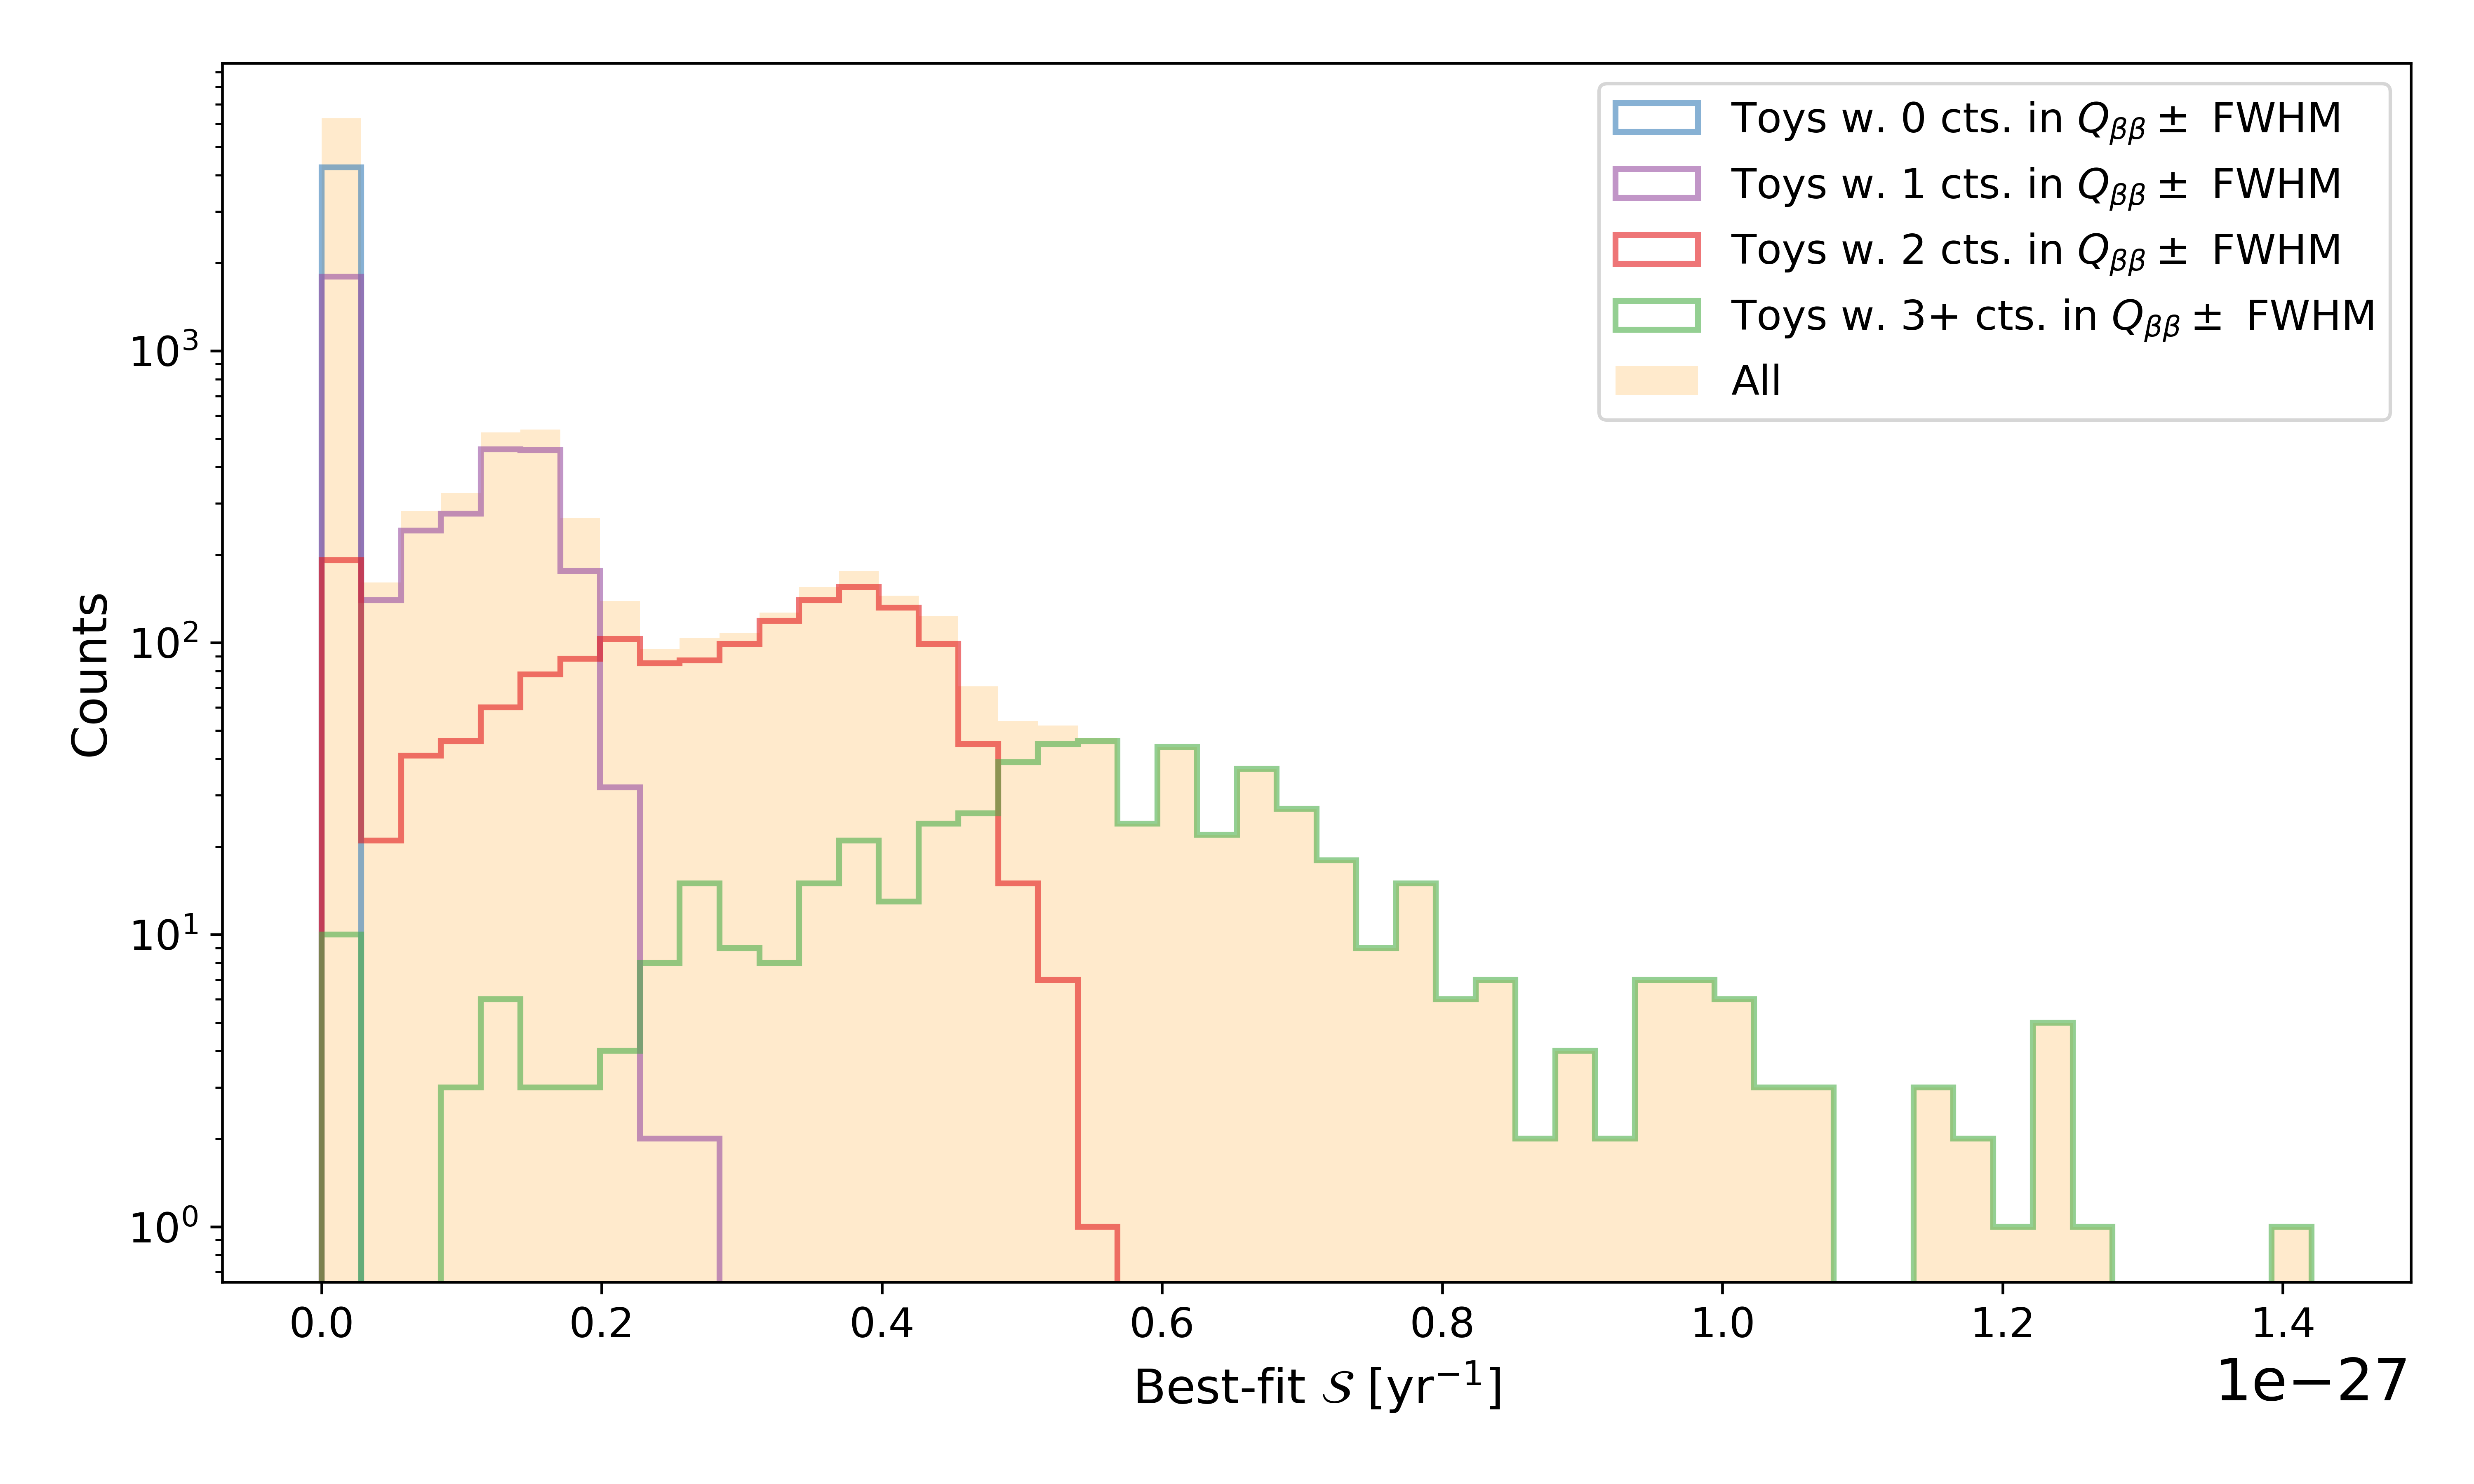
\includegraphics[width=0.9\linewidth]{figures/06_sensitivity/Signal_fits_per_ROIcount.png}
\caption{Distribution of best-fit $\mathcal{S}$ from A/E-based MCMC fits, grouped by the number of events observed within $Q_{\beta \beta} \pm$~FWHM. Modes at non-zero $\mathcal{S}$ are associated with datasets containing one or more background events near the region of interest.} 
\label{fig:S_fit_per_ROIcount}
\end{figure}


This analysis is performed using ZeroNuFit.jl~\cite{dixon_legend-expzeronufitjl_2025}, a specialized Bayesian analysis tool built on the Bayesian Analysis Toolkit (BAT.jl)~\cite{schulz_batjl_2021}. ZeroNuFit.jl implements extended unbinned maximum likelihood fits tailored for $0 \nu \beta \beta$ decay searches, allowing flexible modeling of both signal peaks and background components. The statistical framework we used is further described in~\cite{lnote_25001}. 



\subsection{Results of the Bayesian analysis}

To assess the physics reach of the Transformer PSD strategy, in comparison with the conventional A/E method, a Bayesian half-life sensitivity analysis for the $0 \nu \beta \beta$ decay was performed separately for each PSD method. Using the LEGEND-200 goal exposure and background index, the final $0 \nu \beta \beta$ decay half-life sensitivity of LEGEND-200 was estimated, with the PSD efficiencies treated as Gaussian-distributed nuisance parameters in the fit.  

For each toy dataset, we extracted the 90\% one-sided upper CI limit on the signal half-rate, $\mathcal{S}_{90}$. Its distribution over all toys reflects the expected sensitivity of the experiment: the median, $\tilde{\mathcal{S}}_{90}$ defines the central value, and the 68\% credible interval quantifies the associated uncertainty. This procedure incorporates both statistical fluctuations and systematic uncertainties, as the signal detection efficiency and energy resolution are sampled from their priors and marginalized over in each fit. 
Since the signal half-rate is inversely proportional to the half-life, its median and $68$\% CI range can be directly translated into a median and $68$\% CI range for the $0 \nu \beta \beta$ decay half-life. By comparing the half-lives derived from each PSD method, we can evaluate their respective impacts on the exclusion sensitivity.

\begin{table}
\centering
\caption{Comparison of PSD efficiency, resulting signal half-rate limits and half-life limits for the Transformer and A/E methods.}
\renewcommand{\arraystretch}{1.5}
\begin{tabular}{|| c | c | c | c ||}
	\hline
 	\textbf{Method} & \textbf{PSD eff. [\%]}  & $\boldsymbol{\tilde{\mathcal{S}}_{90} \; [10^{-28} \,\mathrm{yr}^{-1}]}$ & $\mathbf{T^{0 \nu}_{1/2} [10^{27} \, yr]}$ \\
 	\hline
	A/E & $84.3 \pm 0.5$ & $8.23^{+3.65}_{-1.76}$ & $1.22^{+0.33}_{-0.37}$ \\
 	\hline
 	Transformer & $86.7 \pm 1.3$ & $8.00^{+3.42}_{-1.71}$ & $1.25^{+0.34}_{-0.37}$\\
	\hline
\end{tabular}
\label{tab:Results}
\end{table}

All results are summarized in table~\ref{tab:Results}, and the signal half-rate $90$\% CI upper limits distributions are shown in figure~\ref{fig:Results_S_hist}. For the A/E cut, we obtain:

\begin{equation}
    \mathcal{S} = 8.23^{+3.65}_{-1.76} \times 10^{-28} 
\end{equation}

With the definition $T^{0 \nu}_{1/2} = 1/\mathcal{S}$, this translates to a Bayesian 90\% credible lower bound on the $0 \nu \beta \beta$ decay half-life of:

\begin{equation}
    T_{1/2} > 1.22^{+0.33}_{-0.37} \times 10^{27} \; \mathrm{yr}
\end{equation}

Similarly, using the Transformer-based PSD efficiency, the Bayesian analysis yields:

\begin{equation}
    \mathcal{S} < 8.00^{+3.42}_{-1.71} \times 10^{-28} \; \mathrm{yr}^{-1} 
\end{equation}

and

\begin{equation}
    T_{1/2} > 1.25^{+0.34}_{-0.37} \times 10^{27} \; \mathrm{yr} 
\end{equation}

\begin{figure}
\centering
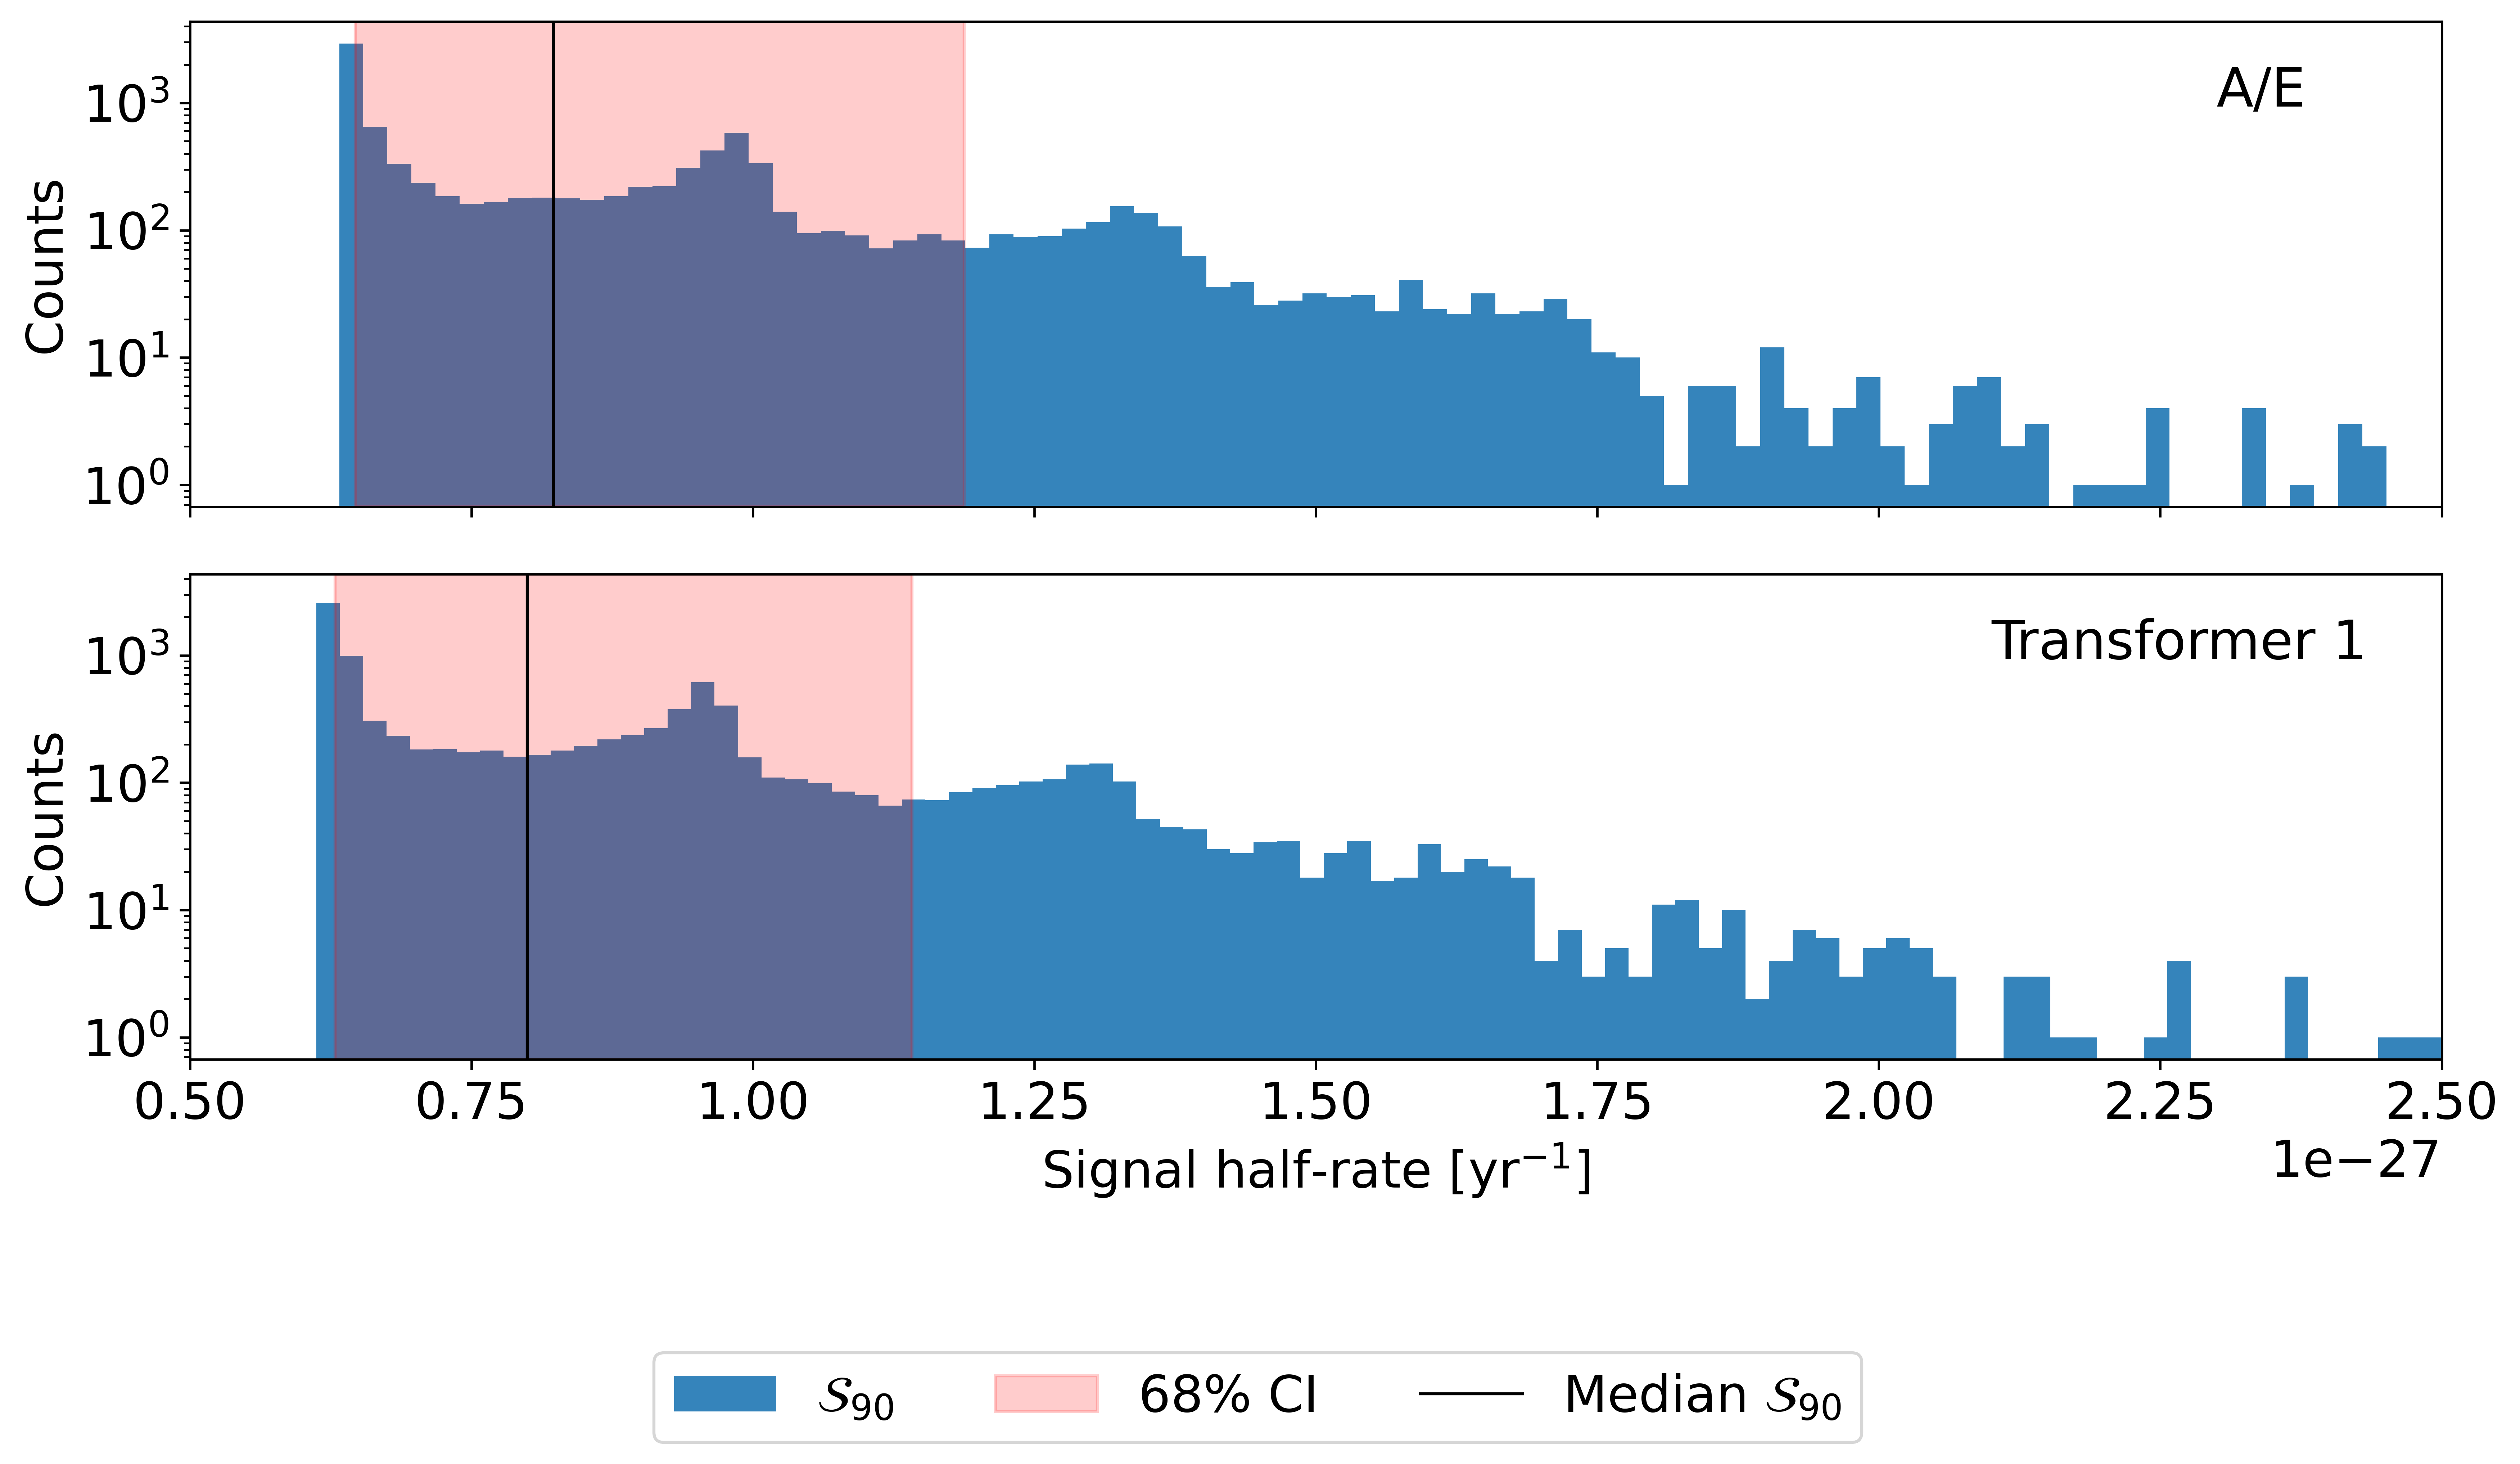
\includegraphics[width=0.9\linewidth]{figures/06_sensitivity/Results_S_histogram_1000kgyr.png}
\caption{Distribution of 90\% upper credible limits on the signal half-rate $\mathcal{S}$ obtained from 10'000 toy Monte Carlo simulations under the background-only hypothesis. The upper plot shows results obtained from the A/E cut, the lower from the Transformer-based PSD cut. The Transformer method achieved a slightly improved sensitivity, reflected by the lower median. } 
\label{fig:Results_S_hist}
\end{figure}